\section{Desenvolvimento Experimental}
\subsection{Materiais e Métodos}
Foi utilizado para o experimento o equipamento PASCO Modelo AP-8210 cosntituido por: 
\begin{itemize}
	\item Câmara  para visualização das gotas graduada em 0,1mm e com placas metálicas em seus terminais;
	\item Anéis para regulagem do foco;
	\item Lâmpada de halogênio;
	\item Filamento de fibra óptica;
	\item Termístor;
	\item Interruptor para controlar o campo elétrico da câmara
	\item Óleo de densidade $886 kg/m^3$.
\end{itemize}

A plataforma deve ser ligada à uma fonte de 500 V em corrente contínua, um multímetro aos terminais de seu termistor e a lâmpada a uma tensão de 12 V DC. Então, se desmonta a câmara para limpeza de sua base com um papel de pequena gramatura, remontando-a novamente. Insere-se a fibra óptica à câmara para regulagem do foco a partir dos aneis sobre a ocular. Por último, borrifa-se o óleo na câmara, fechando-a a partir de uma alavanca em sua lateral. Com o interruptor é possivel ligar o campo entre as placas metálicas.      
\subsection{Dados Obtidos Experimentalmente}
Após a realização do experimento duas vezes, foram obtidos diversos tempos de subida e descida, utilizando os mesmos, foram calculadas as velocidades de subida e descida e também o raio de cada gota, como é possível ver na tabela \ref{tab:Vel}
\begin{table}[!htb]
\centering
\begin{tabular}{l|ll|ll|ll|}

Gota & $Vel_f \times 10^{-5} (m/s)$ & $Delta Vel_f$ & $Vel_r \times 10^{-5} (m/s)$ & $Delta Vel_r$ & $a \times 10^{-7} (m)$ & $Delta a$ \\
\rowcolor[HTML]{C0C0C0} 
1    & 4,31                         & 0,3           & 2,03                         & 0,05          & 4,69                   & 0,03      \\ 
2    & 5,58                         & 0,64          & 1,9                          & 0,01          & 5,21                   & 0,16      \\
\rowcolor[HTML]{C0C0C0} 
3    & 3,11                         & 0,02          & 1,64                         & 0,06          & 4,46                   & 0,04      \\
4    & 0,85                         & 0,63          & 0,6                          & 0,33          & 3,68                   & 0,24      \\
\rowcolor[HTML]{C0C0C0} 
5    & 1,11                         & 0,56          & 0,91                         & 0,25          & 3,09                   & 0,4       \\
6    & 2,22                         & 0,26          & 1,5                          & 0,09          & 3,82                   & 0,21      \\
\rowcolor[HTML]{C0C0C0} 
7    & 0,83                         & 0,63          & 0,53                         & 0,35          & 3,98                   & 0,17      \\
8    & 1,68                         & 0,4           & 0,87                         & 0,26          & 4,5                    & 0,03      \\
\rowcolor[HTML]{C0C0C0} 
9   & 3,5                          & 0,08          & 1,89                         & 0,01          & 4,41                   & 0,05      \\
10   & 4,53                         & 0,36          & 1,93                         & 0,02          & 4,87                   & 0,07      \\ \hline
\end{tabular}
\caption{Valores calculados para as velocidades de descida($V_f$), velocidade de subida($V_r$) e o raio de cada gota($a$), assim como o desvio padrão associado a cada medida.}
\label{tab:Vel}
\end{table}

Com os valores obtidos e  utilizando a equação \ref{eq:14} é possível encontrar o valor de carga que cada gota possui, explicito na tabela \ref{tab:Car}.
\begin{table}[!htb]
\centering
\begin{tabular}{l|ll|}
Gota & $Carga \times 10^{-19} (C)$ & $\Delta Carga$ \\
\rowcolor[HTML]{C0C0C0}
1    & 2,22                        & 0,17           \\ 
2    & 2,99                        & 0,38           \\
\rowcolor[HTML]{C0C0C0} 
3    & 1,41                        & 0,05           \\
4    & 0,22                        & 0,37           \\
\rowcolor[HTML]{C0C0C0} 
5    & 0,35                        & 0,33           \\
6    & 0,93                        & 0,18           \\
\rowcolor[HTML]{C0C0C0} 
7    & 0,2                         & 0,37           \\
8    & 0,55                        & 0,28           \\
\rowcolor[HTML]{C0C0C0} 
9   & 1,7                         & 0,03           \\
10   & 2,32                        & 0,2            \\ \hline
\end{tabular}
\caption{Valores da carga associada a cada gota, assim como o seu respectivo desvio padrão.}
\label{tab:Car}
\end{table}



\subsection{Interpretação dos Resultados}
Utilizando os dados contidos na tabela \ref{tab:Car} é possível produzir o gráfico \ref{im:Car} que contêm a carga pelo número da gota, e assim analisar de forma adequada os dados obtidos.

\begin{figure}[!htb]
	\centering
		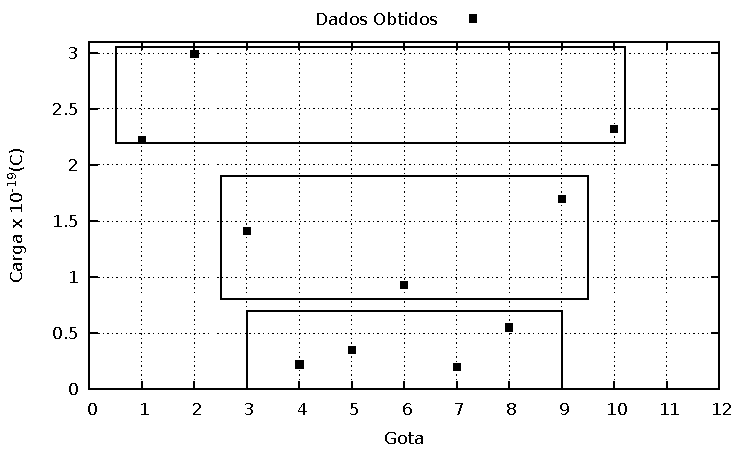
\includegraphics[scale= 1]{grafico/gotas.pdf}
	\caption{Distribuição de carga das gotas.}
	\label{im:Car}
\end{figure}

Analisando o gráfico \ref{im:Car} juntamente com os valores obtidos, temos que as gotas estão separadas em três grupos com um espaçamento regular, um primeiro com as gotas 1,2,10, o segundo grupo com as gotas 3,6,9 e o ultimo grupo com 4,5,7,8. Com isto somos levados a crer que o incremento de carga não é continuo e sim discreto ou quantizado, e este valor pode ser aferido realizando a diferença entre as médias de carga de cada grupo.

\begin{table}[!htb]
\centering
\begin{tabular}{l|l|l|}
Grupo 1 (C)            & Grupo 2 (C)            & Grupo 3 (C)             \\ \hline
\rowcolor[HTML]{C0C0C0} 
$2,51 \times 10^{-19}$ & $1,35 \times 10^{-19}$ & $0,26  \times 10^{-19}$ \\ \hline
\end{tabular}
\caption{Média dos grupos de gotas.}

\end{table}
Fazendo a diferença entre os grupos é obtido o salto médio de $1,12 \times 10^{-19} C$, sendo este o valor de carga de cada elétron obtido pelo experimento. Comparando o valor experimental é obtido 29,90\% de erro em relação ao valor de $e = 1.6021765 \times 10^{-19} C$
